\documentclass{article}
\usepackage{geometry}
\geometry{legalpaper, margin=1in}
\usepackage{amsmath}
\usepackage{amsfonts}
\usepackage{amssymb}
\usepackage{dirtytalk}
\usepackage{xcolor}
\usepackage{cancel}
\usepackage{tikz}
\usetikzlibrary {arrows.meta}
\usetikzlibrary{arrows}

\title{Green's Theorem in Reverse}
\author{OwenTheProgrammer}
\date{July 2025}

\begin{document}

\maketitle

Green's theorem is often used to convert a line integral problem into an equivalent double integral problem. Green's theorem relates a line integral around a simple closed curve $C$ to a double integral over the planar region $R$ bounded by curve $C$. In some cases though, the double integral is a difficult problem, where an equivalent line integral may prove simple. We will go through the steps to utilize \emph{Green's theorem in reverse} in this short document.

\section{Vector Field Parametrization}

We first define a vector field $\vec{F}$ which returns a force acting upon any given Cartesian coordinate $(x, y)$. $\vec{F}$ returns the force vector with component magnitudes relative to the basis vectors $\hat{i}$ and $\hat{j}$. We will parameterize the actions on each basis vector as separate functions $M$ and $N$, given the $x$ and $y$ coordinates.

\begin{equation}\label{eq:VectorField}
    \vec{F}(x, y) = M(x, y)\hat{i} + N(x, y)\hat{j}
\end{equation}

$M(x, y)$ represents the influence in the $\hat{i}$ direction, while $N(x, y)$ represents the influence in the $\hat{j}$ direction.

\section{Green's Theorem}

Green's theorem is defined as such.

\begin{equation}\label{eq:GreensTheorem}
    \oint_C{\vec{F}\cdot d\vec{r}} = \oint_C{\left(M\:dx + N\:dy\right)} = \iint_R{\left(\frac{\partial N}{\partial x} - \frac{\partial M}{\partial y}\right)} dA
\end{equation}

The left integral can be interpreted as the work or \say{effort} done \emph{by} the vector field $\vec{F}$, onto any position $(x, y)$, while taking a infinitesimally small step in direction $d\vec{r}$, along the path $C$.
The \emph{dot product} tracks both the force strength, and how \emph{aligned} the direction $d\vec{r}$ is with the flow of the vector field $\vec{F}$ at position $(x, y)$. This dot product is expanded to the sum of vector components, as shown in the middle integral. The right side reframes the line integral form as the sum of \emph{circulation densities} or the \emph{k-th component of curl} for region $R$. Curl won't be the guiding topic here, but it's defined as the cross product or \emph{outer product} of a vector fields gradient $\nabla$ in basis $\hat{i}, \hat{j}, \hat{k}$.

\begin{equation}\label{eq:kthCurl}
\begin{aligned}
    \textbf{curl}\:\vec{F} &= \nabla\times\vec{F} \\
    &= \left(\frac{\partial P}{\partial y} - \frac{\partial N}{\partial z}\right)\hat{i} - \left(\frac{\partial P}{\partial x} - \frac{\partial M}{\partial z}\right)\hat{j} + \textcolor{blue}{\left(\frac{\partial N}{\partial x} - \frac{\partial M}{\partial y}\right)\hat{k}} \\
    (\textbf{curl}\:\vec{F})\cdot\hat{k} &= \frac{\partial N}{\partial x} - \frac{\partial M}{\partial y}
\end{aligned}
\end{equation}
\emph{The definitions of functions $M$ and $N$ may omit their full signatures for clarity when denoted.}

\section{An Example}
\subsection{Double Integral Method}

Let's execute on an integral that's easy to evaluate for both methods, starting with the traditional double integral method. You may soon notice that this particular example is \emph{much easier} to evaluate through double integration, but \emph{we have different tools for different reasons after all}.

\begin{equation}\label{eq:DoubleIntegralEx1}
    \int_1^2\int_1^2{x^2 + y^2} \:dy\:dx
\end{equation}
Since the rules of \emph{Fubini's theorem} apply here, we may solve by \emph{iterated integration} like so.

\begin{equation}
    \begin{aligned}
        I &= \int_1^2{\left[ \int_1^2{x^2 + y^2} \: dy \right]}\:dx \\
        &= \int_1^2{ \left[ \int_1^2\textcolor{blue}{y^0}x^2 + y^2 \: dy\right]} \:dx && \text{Introduce hidden constant} \\
        &= \int_1^2{ \left[ x^2\int_1^2{y^0\:dy} + \int_1^2 y^2\:dy\right]} \: dx && \text{Separate terms, constant factor} \\
        &= \int_1^2{ \left[ x^2\left[\frac{y^1}{1}\right]_1^2 + \left[\frac{y^3}{3}\right]_1^2 \right]} \: dx && \text{Power rule for integration} \\
        &= \int_1^2{ \left[ x^2 \left[ \frac{2}{1} - \frac{1}{1}\right] + \left[\frac{2^3}{3} - \frac{1^3}{3}\right]\right]} \: dx && \text{F.T.C (Part 2)}\\
        &= \int_1^2{ \left[ x^2 + \frac{7}{3}\right]} \: dx && \text{Evaluate} \\
        &= \int_1^2{ \left[x^2 + \frac{7}{3}\textcolor{blue}{x^0} \right]} \: dx && \text{Introduce hidden constant}\\
        &= \int_1^2 x^2 \: dx + \frac{7}{3}\int_1^2 \: dx && \text{Separate terms, constant factor}\\
        &= \left[\frac{x^3}{3}\right]_1^2 + \frac{7}{3}\left[\frac{x}{1}\right]_1^2 && \text{Power rule for integration} \\
        &= \left[\frac{2^3}{3} - \frac{1^3}{3}\right] + \frac{7}{3}\left[2 - 1\right] = \frac{7}{3} + \frac{7}{3} = \frac{14}{3} + C && \text{Evaluate}
    \end{aligned}
\end{equation}

\begin{equation}\label{eq:DoubleIntegralResult1}
    \int_1^2\int_1^2\left[x^2 + y^2\right]\:dy\:dx = \frac{14}{3} + C
\end{equation}

\subsection{Line Integral Method}

Recall the of the circulation density integral from Green's theorem \eqref{eq:GreensTheorem}\eqref{eq:kthCurl}. We can restructure this integral to match our original double integral \eqref{eq:DoubleIntegralEx1}. First, let's expand the notation to realize the double integrals are the same but abbreviated.

\begin{equation}
    \iint_R{\left(\frac{\partial N}{\partial x} - \frac{\partial M}{\partial y}\right)}\:dA \to \int_a^b\int_c^d{\left(\frac{\partial N}{\partial x} - \frac{\partial M}{\partial y}\right)}\:dy\:dx \quad R \in \left[a, b\right] \times \left[c, d\right]
\end{equation}

To use the relationships proposed in Green's theorem, we must convert our vector field function $\vec{F}$ to an equivalent curl formula \eqref{eq:kthCurl}.

\begin{equation*}
    (\textbf{curl} \: \vec{F}) \cdot \hat{k} = \frac{\partial N}{\partial x} - \frac{\partial M}{\partial y} = x^2 + y^2
\end{equation*}

\begin{center}
\noindent\begin{minipage}{0.4\linewidth}
    \begin{equation*}
        \begin{aligned}
            -\frac{\partial M}{\partial y} &= y^2 \\
            -\int\frac{\partial M}{\partial y}\:dy &= \int{y^2}\:dy \\
            -M &= \frac{y^3}{3} \\
            M(x,y) &= -\frac{y^3}{3}
        \end{aligned}
    \end{equation*}
\end{minipage}
\begin{minipage}{0.4\linewidth}
    \begin{equation*}
        \begin{aligned}
            \frac{\partial N}{\partial x} &= x^2 \\
            \int\frac{\partial N}{\partial x}\:dx &= \int{x^2}\:dx \\
            N(x,y) &= \frac{x^3}{3}
        \end{aligned}
    \end{equation*}%
\end{minipage}
\end{center}

We can verify these function choices will work by deriving to undo the work we did. I'd like to note the fact that there is more than one solution for $N$ and $M$, I've just chosen to cancel the partial derivatives through integration.

\begin{equation*}
\begin{aligned}
    M(x, y) = -x^2 y && N(x, y) = y^2 x
\end{aligned}
\end{equation*}
These choices are equally valid, but we will continue nonetheless. We can verify the the new form is correct by computing the derivatives as laid out in their definition.

\begin{equation*}
\begin{aligned}
    \frac{\partial N}{\partial x} - \frac{\partial M}{\partial y} &= \frac{\partial}{\partial x}\left[\frac{x^3}{3}\right] - \frac{\partial}{\partial y}\left[-\frac{y^3}{3}\right] \\
    &= \frac{1}{\cancel{3}}\left(\cancel{3}x^2\right) - \frac{1}{\cancel{3}}\left(-\cancel{3}y^2\right) \\
    &= x^2 - \left(-y^2\right) \\
    &= x^2 + y^2 \\
    \frac{\partial N}{\partial x} - \frac{\partial M}{\partial y} &= \vec{F}(x, y)
\end{aligned}
\end{equation*}

Now we can comfortably define a line integral with these terms.

\begin{equation}
    \oint_C{\vec{F}\cdot d\vec{r}} = \oint_C{\left(M\:dx + N\:dy\right)} = \oint_C{\left(\left[-\frac{y^3}{3}\right]\:dx + \left[\frac{x^3}{3}\right]\:dy\right)}
\end{equation}

\subsubsection{Piecewise Linear Sum}

The diagram in Figure 1 visualizes the bounding segments around region $R$. Technically, the region is defined entirely by curve $C$, but because this region is simple and closed, we can represent the entire curve as a sum of segments. It is \emph{imperative} to evaluate the curve \emph{counter-clockwise}, since the curl vector will face backwards if the direction is reversed.

\begin{center}
    
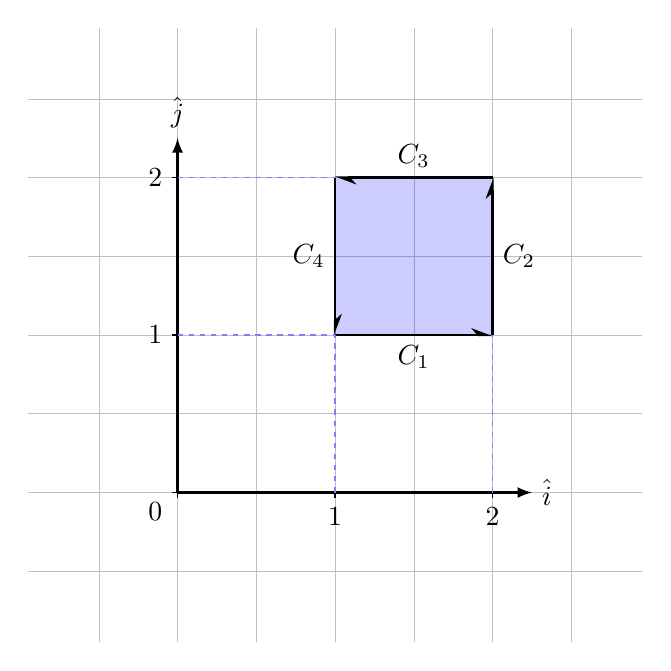
\begin{tikzpicture}
    \coordinate (0) at (2,2);
    \coordinate (1) at (4,2);
    \coordinate (2) at (4,4);
    \coordinate (3) at (2,4);
    \draw[step=1cm,gray!50,very thin] (-1.9,-1.9) grid (5.9,5.9);
    \draw[thick,-latex] (0,0) -- (4.5, 0) node[anchor=west] {$\hat{i}$};
    \draw[thick,-latex] (0,0) -- (0, 4.5) node[anchor=south] {$\hat{j}$};
    % Draw the grid markers
    \foreach \x in {1, 2} \draw (\x*2 cm,2pt) -- (\x*2 cm,-2pt) node[anchor=north] {$\x$};
    \foreach \y in {1, 2} \draw (2pt, \y*2 cm) -- (-2pt, \y*2 cm) node[anchor=east] {$\y$};
    \draw (0,2pt) -- (0, -2pt);
    \draw (2pt,0) -- (-2pt, 0) node[anchor=north east] {$0$};
    % Draw the parameter space
    \draw[fill=blue, opacity=0.2] (0) -- (1) -- (2) -- (3) -- cycle;
    \draw[thick,-{Stealth[left]}] (0) -- (1) node[midway, below] {$C_1$};
    \draw[thick,-{Stealth[left]}] (1) -- (2) node[midway, right] {$C_2$};
    \draw[thick,-{Stealth[left]}] (2) -- (3) node[midway, above] {$C_3$};
    \draw[thick,-{Stealth[left]}] (3) -- (0) node[midway, left] {$C_4$};
    \draw[-,thin,blue!50,dash pattern=on 2pt off 2pt] (2, 0) -- (0);
    \draw[-,thin,blue!50,dash pattern=on 2pt off 2pt] (4, 0) -- (1);
    \draw[-,thin,blue!50,dash pattern=on 2pt off 2pt] (0, 4) -- (3);
    \draw[-,thin,blue!50,dash pattern=on 2pt off 2pt] (0, 2) -- (0);
\end{tikzpicture}\break
\textsubscript{Figure 1}
\end{center}

Because our region is square in shape, we will have four segments in total. As mentioned beforehand, the sum of those segments will represent the entire curve \emph{en masse}.

\begin{equation}
    \oint_C{\vec{F}\cdot d\vec{r}} = \sum_{i=1}^4{\oint_{C_i}{\vec{F}\cdot d\vec{r}}}
\end{equation}

To convert our segments to integrable lines, we need to parameterize the domain of each segment $C_n$ as a parametric vector $\vec{r}_n$, dependent on $t$. In essence, we are doing a \emph{change of variables} to make components $x$ and $y$ linearly dependent on $t$. We can also bring the derivatives $dx$ and $dy$ to the $dt$ world. 

We define these vectors based on the endpoints we want for given values $t_0$ and $t_1$ through \emph{linear interpolation}. For example, $C_1$ is a vector constrained by the following.

\begin{equation*}
    \begin{aligned}
        \vec{r}_1(t_0) &= (\textcolor{red}{1}, \textcolor{blue}{1}) && \vec{r}_1(t_1) = (\textcolor{red}{2}, \textcolor{blue}{1}) \\
        \vec{r}_1(t=1) &= \textcolor{red}{1\:\hat{i}} + \textcolor{blue}{1\:\hat{j}} &&
        \vec{r}_1(t=2) = \textcolor{red}{2\:\hat{i}} + \textcolor{blue}{1\:\hat{j}} \\
        f_x(t) &= 
        \begin{cases}
            1 & t=1 \\
            2 & t=2
        \end{cases}
        &&
        f_y(t) = \begin{cases}
            1 & t=1 \\
            1 & t=2
        \end{cases} \\
        f_x(t) &= t && f_y(t) = 1 \\
        \vec{r}_1(t) &= t\:\hat{i} + 1\:\hat{j}
    \end{aligned}
\end{equation*}

The left section of the following holds each segment $C_n$ as the parameterized vector $\vec{r}_n$, used for the corresponding line integrals on the right.
\begin{center}
\noindent\begin{minipage}{0.4\linewidth}
    \begin{equation*}
    \begin{aligned}
        \vec{r}_1(t) &= t\:\hat{i} + 1\:\hat{j} && t \in \left[1, 2\right] \\
        x &= t && y = 1 \\
        dx &= 1\:dt && dy = 0\:dt
    \end{aligned}
    \end{equation*}
    \begin{equation*}
    \begin{aligned}
        M(x,y) &= \frac{-y^3}{3} \to \frac{-1^3}{3} \\
        N(x,y) &= \frac{x^3}{3} \to \frac{t^3}{3}
    \end{aligned}
    \end{equation*}
\end{minipage}
\begin{minipage}{0.4\linewidth}
    \begin{equation*}
    \begin{aligned}
            C_1 &= \int_1^2{\left( M\:dx + N\:dy \right)} \\
            &= \int_1^2{ \left( \left[\frac{-1^3}{3}\right] \left( 1\:dt \right) + \cancel{\left[\frac{t^3}{3}\right] \left( 0\:dt \right)} \right)} \\
            &= \int_1^2{ \left(\frac{-1}{3}\right) \: dt} \\
            &= \frac{-1}{3}\int_1^2{\textcolor{blue}{t^0}\:dt} = \frac{-1}{3}\left[\frac{t}{1}\right]_1^2
            = \frac{-1}{3}\left[2 - 1\right] \\
            &= \frac{-1}{3} + C \\
    \end{aligned}
    \end{equation*}
    \end{minipage}
\end{center}

\begin{center}
\noindent\begin{minipage}{0.4\linewidth}
    \begin{equation*}
    \begin{aligned}
        \vec{r}_2(t) &= 2\:\hat{i} + t\:\hat{j} && t \in \left[1, 2\right] \\
        x &= 2 && y = t \\
        dx &= 0\:dt && dy = 1\:dt
    \end{aligned}
    \end{equation*}
    \begin{equation*}
    \begin{aligned}
        M(x,y) &= \frac{-y^3}{3} \to \frac{-t^3}{3} \\
        N(x,y) &= \frac{x^3}{3} \to \frac{2^3}{3}
    \end{aligned}
    \end{equation*}
\end{minipage}
\begin{minipage}{0.4\linewidth}
    \begin{equation*}
    \begin{aligned}
        C_2 &= \int_1^2{\left( M\:dx + N\:dy\right)} \\
        &= \int_1^2{\left( \cancel{\left[\frac{-t^3}{3}\right] \left(0\:dt\right)} + \left[\frac{2^3}{3}\right]\left(1\:dt\right)\right)} \\
        &= \int_1^2{\left(\frac{2^3}{3}\right) \: dt} \\
        &= \frac{8}{3}\int_1^2{\textcolor{blue}{t^0}\:dt} = \frac{8}{3}\left[\frac{t}{1}\right]_1^2 \\
        &= \frac{8}{3}\left[2 - 1\right] = \frac{8}{3} + C
    \end{aligned}
    \end{equation*}
\end{minipage}
\end{center}

\begin{center}
\noindent\begin{minipage}{0.4\linewidth}
    \begin{equation*}
    \begin{aligned}
        \vec{r}_3(t) &= -t\:\hat{i} + 2\:\hat{j} && t \in \left[1, 2\right] \\
        x &= -t && y = 2 \\
        dx &= -1\:dt && dy = 0\:dt
    \end{aligned}
    \end{equation*}
    \begin{equation*}
    \begin{aligned}
        M(x, y) &= \frac{-y^3}{3} \to \frac{-2^3}{3} \\
        N(x, y) &= \frac{x^3}{3} \to \frac{-t^3}{3}
    \end{aligned}
    \end{equation*}
\end{minipage}
\begin{minipage}{0.4\linewidth}
    \begin{equation*}
    \begin{aligned}
        C_3 &= \int_1^2{\left(M\:dx + N\:dy\right)} \\
        &= \int_1^2{\left(\left[\frac{-2^3}{3}\right]\left(-1\:dt\right) + \cancel{\left[\frac{-t^3}{3}\right]\left(0\:dt\right)}\right)} \\
        &= \frac{8}{3}\int_1^2{\textcolor{blue}{t^0}\:dt} = \frac{8}{3}\left[\frac{t}{1}\right]_1^2 = \frac{8}{3}\left[2 - 1\right] \\
        &= \frac{8}{3} + C
    \end{aligned}
    \end{equation*}
\end{minipage}
\end{center}

\begin{center}
\noindent\begin{minipage}{0.4\linewidth}
    \begin{equation*}
    \begin{aligned}
    \vec{r}_4(t) &= 1\:\hat{i} - t\:\hat{j} && t \in \left[1, 2\right] \\
    x &= 1 && y = -t \\
    dx &= 0\:dt && dy = -1\:dt
    \end{aligned}
    \end{equation*}
    \begin{equation*}
    \begin{aligned}
        M(x,y) &= \frac{-y^3}{3} \to \frac{t^3}{3} \\
        N(x,y) &= \frac{x^3}{3} \to \frac{1^3}{3}
    \end{aligned}
    \end{equation*}
\end{minipage}
\begin{minipage}{0.4\linewidth}
    \begin{equation*}
    \begin{aligned}
        C_4 &= \int_1^2{\left(M\:dx + N\:dy\right)} \\
        &= \int_1^2{\left( \cancel{\left[\frac{t^3}{3}\right]\left(0\:dt\right)} + \left[\frac{1^3}{3}\right]\left(-1\:dt\right) \right)} \\
        &= \int_1^2{ \left(\frac{-1^3}{3}\right)\:dt} \\
        &= \frac{-1}{3}\int_1^2{ \textcolor{blue}{t^0}\:dt} = \frac{-1}{3}\left[\frac{t}{1}\right]_1^2 = \frac{-1}{3}\left[2 - 1\right] \\
        &= \frac{-1}{3} + C
    \end{aligned}
    \end{equation*}
\end{minipage}
\end{center}

Finally, the sum of all integrated segments work out to be equivalent to the double integral result \eqref{eq:DoubleIntegralResult1}.

\begin{equation}
    \begin{aligned}
        \sum_{i=1}^4{\oint_{C_i}{\vec{F}\cdot d\vec{r}}} &= C_1 + C_2 + C_3 + C_4 \\
        &= \frac{-1}{3} + \frac{8}{3} + \frac{8}{3} + \frac{-1}{3} \\
        &= \frac{14}{3} + C
    \end{aligned}
\end{equation}

\end{document}
